

\section{Introduction}

The {\bf spatial searching} package implements
exact and approximate distance browsing
by providing implementations of algorithms supporting

\begin{itemize} 

\item
both nearest and furthest neighbor searching

\item
both exact and approximate searching

\item
(approximate) range searching

\item 
(approximate) $k$-nearest and $k$-furthest neighbor searching

\item 
(approximate) incremental nearest and incremental furthest neighbor searching

\item
query items representing points and spatial objects.

\end{itemize}

In these searching problems a set $P$ of data points in
$d$-dimensional space is given.  The points can be represented by
Cartesian coordinates or homogeneous coordinates.  These points are
preprocessed into a $k$-$d$ tree data structure, so that given any
query item $q$ the points of $P$ can be browsed efficiently.  The
approximate spatial searching package is designed for data sets that
are small enough to store the search structure in main memory (in
contrast to approaches from databases that assume that the data reside
in secondary storage).

\subsection{Neighbor Searching}

Spatial searching supports browsing through a collection of
$d$-dimensional spatial objects stored in a spatial data structure on
the basis of their distances to a query object. The query object may
be a point or an arbitrary spatial object, e.g a $d$-dimensional
sphere. The objects in the spatial data structure are $d$-dimensional
points.

Often the number of the neighbors to be computed is not know
beforehand, e.g. because the number may depend on some properties of
the neighbors (e.g. when querying for the nearest city to Paris with
population greater than a million) or the distance to the query point.
The convential approach is $k$-{\bf nearest neighbor searching} that
makes use of a $k$-nearest neighbor algorithm, where $k$ is known
prior to the invocation of the algorithm.  Hence, the number of
nearest neighbors has to be guessed. If the guess is too large
redundant computations are performed.  If the number is too small the
computation has to be reinvoked for a larger number of neighbors,
thereby performing redundant computations.  Therefore, Hjaltason and
Samet \cite{hs-rsd-95} introduced {\bf incremental nearest neighbor
searching} in the sense that having obtained the $k$ nearest
neighbors, the $k$ + 1$^{st}$ neighbor can be obtained without having
to calculate the $k$ + 1 nearest neighbor from scratch.
 

Spatial searching typically consists of a preprocessing phase and a
searching phase.  In the preprocessing phase one builds a search
structure and in the searching phase one makes the queries.  In the
preprocessing phase the user builds a $k$-$d$ tree data structure
storing the spatial data.  In the searching phase the user invokes a
searching method to browse the spatial data.

With relatively minor modifications, nearest neighbor searching
algorithms can be used to find the furthest object from the query
object.  Therefore, {\bf furthest neighbor searching} is also
supported by the spatial searching package.

The execution time for exact neighbor searching can be reduced by
relaxing the requirement that the neighbors should be computed
exactly.  If the distances of two objects to the query object are
approximately the same, instead of computing the nearest/furthest
neighbor exactly, one of these objects may be returned as the
approximate nearest/furthest neighbor. I.e., given some non-negative
constant $\epsilon$ the distance of an object returned as an
approximate $k$-nearest neighbor must not be larger than
$(1+\epsilon)r$, where $r$ denotes the distance to the real $k^{th}$
nearest neighbor.  Similar the distance of an approximate $k$-furthest
neighbor must not be smaller than $r/(1+\epsilon)$.  Obviously, for
$\epsilon=0$ we get the exact result, and the larger $\epsilon$ is,
the less exact the result.

\subsection{Range searching}

{\bf Exact range searching} and {\bf approximate range searching} is
supported using exact or fuzzy $d$-dimensional objects enclosing a
region.  The fuzziness of the query object is specified by a parameter
$\epsilon$ denoting a maximal allowed distance to the boundary of a
query object.  If the distance to the the boundary is at least
$\epsilon$, points inside the object are always reported and points
outside the object are never reported. Points within distance
$\epsilon$ to the boundary may be or may be not reported.  For exact
range searching the fuzziness parameter $\epsilon$ is set to zero.

\subsection{The $k$-$d$ tree}
\label{Kd_tree_section}

Bentley \cite{b-mbstu-75} introduced the $k$-$d$ tree as a
generalization of the binary search tree in higher dimensions. $k$-$d$
trees hierarchically decompose space into a relatively small number of
rectangles such that no rectangle contains too many input objects.
For our purposes, a {\it rectangle} in real $d$ dimensional space,
$\R^d$, is the product of $d$ closed intervals on the coordinate axes.
$k$-$d$ trees are obtained by partitioning point sets in $\R^d$ using
($d$-1)-dimensional hyperplanes.  Each node in the tree is split into
two children by one such separating hyperplane.  Several splitting
rules (see Section \ref{Spatial_Searching:Splitting_rule_section} can
be used to compute a seperating ($d$-1)-dimensional hyperplane.

Each internal node of the $k$-$d$ tree is associated with a rectangle
and a hyperplane orthogonal to one of the coordinate axis, which
splits the rectangle into two parts.  Therefore, such a hyperplane,
defined by a splitting dimension and a splitting value, is called a
separator.  These two parts are then associated with the two child
nodes in the tree. The process of partitioning space continues until
the number of data points in the rectangle falls below some given
threshold. The rectangles associated with the leaf nodes are called
{\it buckets}, and they define a subdivision of the space into
rectangles.  Data points are only stored in the leaf nodes of the
tree, not in the internal nodes.

Friedmann, Bentley and Finkel \cite{fbf-afbml-77} described the
standard search algorithm to find the $k$th nearest neighbor by
searching a $k$-$d$ tree recursively.

When encountering a node of the tree, the algorithm first visits the
child that is closest to the query point. On return, if the rectangle
containing the other child lies within 1/ (1+$\epsilon$) times the
distance to the $k$th nearest neighbors so far, then the other child
is visited recursively.  Priority search \cite{am-annqf-93} visits the
nodes in increasing order of distance from the queue with help of a
priority queue.  The search stops when the distance of the query point
to the nearest nodes exceeds the distance to the nearest point found
with a factor 1/ (1+$\epsilon$).  Priority search supports next
neighbor search, standard search does not.

In order to speed-up the internal distance computations in nearest
neighbor searching in high dimensional space, the approximate
searching package supports orthogonal searching. Orthogonal searching
implements the efficient incremental distance computation technique
introduced by Arya and Mount \cite{am-afvq-93}.  Orthogonal searching
works only for neighbor queries with query items represented as points
and with a quadratic form distance, defined by $d_A(x,y)=
(x-y)A(x-y)^T$, where the matrix $A$ is positive definite,
i.e. $d_A(x,y) \geq 0$.  An important class of quadratic form
distances are weighted Minkowski distances.  Given a parameter $p>0$
and parameters $w_i \geq 0, 0 < i \leq d$, the weighted Minkowski
distance is defined by $l_p(w)(r,q)= ({\Sigma_{i=1}^{i=d} \,
w_i(r_i-q_i)^p})^{1/p}$ for $0 < p <\infty$ and defined by
$l_{\infty}(w)(r,q)=max \{w_i |r_i-q_i| \mid 1 \leq i \leq d\}$.  The
Manhattan distance ($p=1$, $w_i=1$) and the Euclidean distance ($p=2$,
$w_i=1$) are examples of a weighted Minkowski metric.

To speed up distance computations also transformed distances are used
instead of the distance itself.  For instance for the Euclidean
distance, to avoid the expensive computation of square roots, squared
distances are used instead of the Euclidean distance itself.


\section{Example Programs}

We give six examples.  The first example illustrates nearest neighbor
searching.  The second example illustrates selecting a splitting rule.
The third is an example of approximate furthest neighbor searching
using a $d$-dimensional iso-rectangle as an query object.  Approximate
range searching is illustrated by the fourth example.  The fifth
example illustrates distance browsing and the last example illustrates
nearest and furthest neighbour searching using a user defined point
and distance class.

\subsection{Example of Nearest Neighbor Searching}

The first example illustrates nearest neighbor searching. The random
data points are preprocessed in a $k$-$d$ tree. For each of the random
query points its nearest neighbor is obtained.  In this example the
Euclidean distance is used by default. To avoid the expensive
computation of square roots, the nearest neighbor searching algorithm
computes squared distances instead of the Euclidean distance itself.
Finally, if the Euclidean distance is reported the square root is
taken.

\ccIncludeExampleCode{../../examples/Spatial_searching/Nearest_neighbor_searching.C}

\subsection{Example of selecting a splitting rule and setting the bucket size.}

This example program illustrates selecting a splitting rule and
setting the maximal allowed bucket size.  The only differences with
the previous example are the definition of the traits class, where
Fair is selected as a splitting rule, and the declaration of a
variable \ccc{tr} of type TreeTraits, needed to set the maximal
allowed bucket size.

\ccIncludeExampleCode{../../examples/Spatial_searching/Using_fair_splitting_rule.C}

\subsection{Example of General Neighbor Searching}

This example program illustrates approximate nearest and furthest
neighbor searching using 4-dimensional Cartesian coordinates.  Five
approximate nearest and furthest neighbors of the query rectangle
$[0.1,0.2]^4$ are computed.
 
\ccIncludeExampleCode{../../examples/Spatial_searching/General_neighbor_searching.C}

\subsection{Example of a Range Query}

This example program illustrates approximate range querying for
4-dimensional fuzzy iso-rectangles and spheres using homogeneous
coordinates.

\ccIncludeExampleCode{../../examples/Spatial_searching/Fuzzy_range_query.C}


\subsection{Example of distance browsing}

This example program illustrates distance browsing for $4$-dimensional
points with a positive first coordinate using orthogonal priority
search.

 
\ccIncludeExampleCode{../../examples/Spatial_searching/Distance_browsing.C}


\subsection{Example illustrating use of user defined point and distance class}

In this example the user provides an implementation of 3-dimensional points and an
implementation of the Euclidean distance.

\ccIncludeExampleCode{../../examples/Spatial_searching/User_defined_point_and_distance.C}

\section{Software design}

\begin{ccTexOnly}
\begin{figure}[t]
\begin{center}
\leavevmode
\vspace*{-6.5cm}
\hspace*{-2cm}
\scalebox{.3}{\includegraphics{Fig1.ps}}
\end{center}
\vspace*{6cm}
\caption{Scheme of concepts and classes implementing neighbor searching algorithms.
Point is used as shorthand for SpatialPoint, Tree is used as shorthand for SpatialTree,
Container is used as shorthand for PointContainer,
Separator is used as shorthand for SpatialSeparator,
and Distance as shorthand for both GeneralDistance and OrthogonalDistance.
\label{ASPAS:Fig1}}
\end{figure}
\end{ccTexOnly}

\begin{ccHtmlOnly}

<P>
<center>
<img border=0 src="./Fig1.gif" alt=" "><br> 
Scheme of concepts and classes implementing neighbor searching algorithms.
Point is used as shorthand for SpatialPoint, Tree is used as shorthand for SpatialTree,
Container is used as shorthand for PointContainer, Separator is used as shorthand for SpatialSeparator,
and Distance as shorthand for both GeneralDistance and OrthogonalDistance.
</center>

\end{ccHtmlOnly}

The spatial searching package consists of a number of concepts, each implemented by
one or more classes, and four classes implementing neighbor 
searching algorithms. 
\begin{ccTexOnly}
(See figure \ref{ASPAS:Fig1}) 
\end{ccTexOnly}

\subsection{Concepts}

The concepts related to the spatial searching package are

\begin{itemize}

\item
\ccc{QueryItem} denoting a $d$-dimensional spatial query object. The concepts
\ccc{SpatialPoint}, \ccc{IsoBox_d}, and \ccc{Ball_d} refine \ccc{QueryItem}.

\item 
\ccc{SpatialPoint} 
denoting a $d$-dimensional point, as implemented by 
\ccc{CGAL::Point_2<Kernel>}, \ccc{CGAL::Point_3<Kernel>}, and \ccc{CGAL::Point_d<Kernel>}.

\item
\ccc{IsoBox_d} 
denoting a $d$-dimensional iso-box, as implemented
by
\ccc{CGAL::Iso_rectangle_2<Kernel>}, \ccc{CGAL::Iso_cuboid_3<Kernel>}, 
and \ccc{CGAL::Iso_box_d<Kernel>}.

\item
\ccc{Ball_d}
denoting a $d$-dimensional ball, as implemented by
\ccc{CGAL::Circle_2<Kernel>}, \ccc{CGAL::Sphere_3<Kernel>},
and \ccc{CGAL::Sphere_d<Kernel>}.


\item
\ccc{PointContainer} denoting a container, that stores points and
provides method to support the implementation of splitting rules. 
\ccc{CGAL::Point_container<SpatialPoint>} provides an implementation.


\ccc{SpatialSeparator} denoting a $d-1$-dimensional
subspace separating a $d$-dimensional spaces in two parts,
as implemented by \ccc{CGAL::Plane_separator<NT>}.

\item 
\ccc{Splitter} denoting a splitting rule as implemented by the function object classes 
\ccc{CGAL::Midpoint_of_rectangle<SpatialPoint, PointContainer, SpatialSeparator>},
\ccc{CGAL::Midpoint_of_max_spread<SpatialPoint, PointContainer, SpatialSeparator>},
\ccc{CGAL::Sliding_midpoint<SpatialPoint, PointContainer, SpatialSeparator>},
\ccc{CGAL::Median_of_rectangle<SpatialPoint, PointContainer, SpatialSeparator>},
\ccc{CGAL::Median_of_max_spread<SpatialPoint, PointContainer, SpatialSeparator>},
\ccc{CGAL::Fair<SpatialPoint, PointContainer, SpatialSeparator>}, and
\ccc{CGAL::Sliding_Fair<SpatialPoint, PointContainer, SpatialSeparator>}.

\item
\ccc{TreeTraits} denoting a traits class for the construction of a tree.
\ccc{CGAL::Kd_tree_traits_point< SpatialPoint, Splitter >} provides an implementation. 

\item
\ccc{GeneralDistance} denoting a general distance object. A general distance object should define distances between a query object
and the points stored in a tree and between the query object and the rectangles associated with the nodes from the tree.
Implementations for queries defined by points are provided
by \ccc{CGAL::Euclidean_distance<SpatialPoint>}, and
\ccc{CGAL::Weighted_Minkowski_distance<SpatialPoint>} implementing 
a weighted Minkowski metric.

An implementation for queries defined by rectangles is provided by
\ccc{CGAL::Manhattan_distance_rectangle_point<IsoBox_d,SpatialPoint>}.
An implementation for queries defined by spheres is provided by
\ccc{CGAL::Euclidean_distance_sphere_point<Ball_d,SpatialPoint>}.

\item
\ccc{OrthogonalDistance} denoting a distance object. An orthogonal distance object should define distances 
between a query object and the points stored in a tree and between the
query object and the rectangles associated with the nodes from the
tree.  Also, incremental distance computation is supported by an
orthogonal distance object.  Implementations for queries defined by
points are provided by \ccc{CGAL::Euclidean_distance<SpatialPoint>},
and
\ccc{CGAL::Weighted_Minkowski_distance<SpatialPoint>} implementing 
a weighted Minkowski metric.

\item
\ccc{SpatialTree} denoting a tree supporting spatial searching 
\ccc{CGAL::Kd_tree<TreeTraits>} provides an implementation of $k$-$d$ trees.

\end{itemize}

\subsection{Neighbor search}

The four classes implementing neighbor searching algorithms are

\begin{itemize}

\item
The class \ccc{CGAL::General_standard_search<TreeTraits, Distance, QueryItem, SpatialTree>} 
implementing the standard search strategy for general distances
like the Manhattan distance for iso-rectangles.
Requires no use of extended nodes in the $k$-$d$ tree and supports only $k$
neighbor searching for queries defined by points or spatial objects.


\item
The class \ccc{CGAL::General_priority_search<TreeTraits, GeneralDistance, QueryItem, SpatialTree>} implementing the priority search 
strategy for general distances
like the Manhattan distance for iso-rectangles.
Requires no use of extended nodes in the $k$-$d$ tree and supports incremental
neighbor searching and distance browsing for queries defined by points or spatial objects.

\item
The class \ccc{CGAL::Orthogonal_standard_search<TreeTraits, OrthogonalDistance, SpatialTree>} implementing the standard search strategy for 
orthogonal distances
like a weighted Minkowski distance. Requires the use of extended nodes in the $k$-$d$ tree and supports 
only $k$ neighbor searching for point queries.

\item
The class \ccc{Orthogonal_priority_search<TreeTraits, GeneralDistance, QueryItem, SpatialTree>} implementing the priority search strategy for general 
distances
like a weighted Minkowski distance. Requires the use of extended nodes in the $k$-$d$ tree and supports incremental
neighbor searching and distance browsing for point queries.

\end{itemize}

If one wants to implement a splitter or a tree data structure
methods from the following classes can be used

\begin{itemize}

\item
The class \ccc{CGAL::Kd_tree_rectangle<NT>} implementing $d$-dimensional iso-rectangles, 
methods to compute bounding boxes
of point sets and methods to split iso-rectangles.

\item
The class \ccc{CGAL::Kd_tree_node<TreeTraits>} implementing $k$-$d$ tree nodes.

\end{itemize}

\subsection{Range searching}

Besides neighbor searching descirbed above, the spatial searching package
supports also range searching using the method \\
\ccc{template <class OutputIterator, class FuzzyQueryItem>} \\
\ccc{OutputIterator CGAL::Kd_tree<Treetraits>::search(OutputIterator it, const FuzzyQueryItem& q)}.\\
Implementations for the concept \ccc{FuzzyQueryItem} are provided by
the class \ccc{CGAL::Fuzzy_iso_box_d<SpatialPoint, IsoBox_d>}  
and the class \ccc{CGAL::Fuzzy_sphere_d<SpatialPoint>}. 
For range searching of large data sets the user may set the parameter \ccc{bucket_size} 
used in building the $k$-$d$ tree to a large value (e.g. 100), 
because in general the query time will be less then using the default value 5 for the parameter \ccc{bucket_size}.


\section{Splitting Rules}
\label{Spatial_Searching:Splitting_rule_section}

Instead of using the default splitting rule \ccc{Sliding_midpoint} described below,
a user may, depending upon the data, select 
one from the following splitting rules,
which determine how a separating hyperplane is computed:

\begin{itemize}

\item \ccc{Midpoint_of_rectangle}

This splitting rule cuts a rectangle through its midpoint orthogonal
to the longest side.

\item \ccc{Midpoint_of_max_spread}

This splitting rule cuts a rectangle through $(Mind+Maxd)/2$ orthogonal
to the dimension with the maximum point spread $[Mind,Maxd]$.

\item \ccc{Sliding_midpoint}

This is a modification of the midpoint of rectangle splitting rule.
It first attempts to perform a midpoint of rectangle split as
described above. If data points lie on both sides of the separating
plane the sliding midpoint rule computes the same separator as
the midpoint of rectangle rule. If the data points lie only on one
side it avoids this by sliding the separator, computed by
the midpoint of rectangle rule, to the nearest datapoint.

\item \ccc{Median_of_rectangle}

The splitting dimension is the dimension of the longest side of the rectangle.
The splitting value is defined by the median of the coordinates of the data points
along this dimension.

\item \ccc{Median_of_max_spread}

The splitting dimension is the dimension of the longest side of the rectangle.
The splitting value is defined by the median of the coordinates of the data points
along this dimension.

\item \ccc{Fair}

This splitting rule is a compromise between the median of rectangle
splitting rule and the midpoint of rectangle splitting rule. This
splitting rule maintains an upper bound on the maximal allowed ratio
of the longest and shortest side of a rectangle (the value of this
upper bound is set in the constructor of the fair splitting
rule). Among the splits that satisfy this bound, it selects the one in
which the points have the largest spread.  It then splits the points
in the most even manner possible, subject to maintaining the bound on
the ratio of the resulting rectangles.

\item \ccc{Sliding_fair}

This splitting rule is a compromise between the fair splitting rule
and the sliding midpoint rule.  Sliding fair-split is based on the
theory that there are two types of splits that are good: balanced
splits that produce fat rectangles, and unbalanced splits provided the
rectangle with fewer points is fat.

Also, this splitting rule maintains an upper bound on the maximal
allowed ratio of the longest and shortest side of a rectangle (the
value of this upper bound is set in the constructor of the fair
splitting rule). Among the splits that satisfy this bound, it selects
the one one in which the points have the largest spread.  It then
considers the most extreme cuts that would be allowed by the aspect
ratio bound. This is done by dividing the longest side of the
rectangle by the aspect ratio bound. If the median cut lies between
these extreme cuts, then we use the median cut. If not, then consider
the extreme cut that is closer to the median.  If all the points lie
to one side of this cut, then we slide the cut until it hits the first
point.  This may violate the aspect ratio bound, but will never
generate empty cells.

\end{itemize}



\section{Backward compability with the Kd-trees package}
\label{Spatial_searching:Backward_compability_Kd-trees}

In release 2.3 of CGAL
$k$-$d$ trees have been implemented by the class \ccc{CGAL::Kdtree_d<TreeTraits>}, 
that is parameterized with one of the
traits classes 

\begin{itemize}

\item
\ccc{Kd_Interface} supporting user defined $d$-dimensional points.

\item 
\ccc{Kd_Interface_2d} supporting \ccc{CGAL::Point_2<R>}. 

\item
\ccc{Kd_Interface_3d} supporting \ccc{CGAL::Point_3<R>}. 

\end{itemize}

This $k$-$d$ tree implementation is backward compatible with the
$k$-$d$ tree implementation provided by the spatial searching package,
except for the definition of \ccc{Kdtree_d<Traits>::Box} and for the
requirements on the definition of user defined $d$-dimensional points.

In contrast with the old $k$-$d$ tree implementation, the spatial searching package
requires that the \ccc{Kdtree_d<Traits>::Box} is bounded.

The user can move from the old $k$-$d$ tree implementation to the spatial searching package by
replacing in the code \\
\begin{verbatim}
#include <CGAL/Kd_tree_d.h>
by
#include <CGAL/Kd_tree_d_new.h>
\end{verbatim}
 
Further, the spatial searching package requires that the user provides
for a user defined point class \ccc{My_Point} a nested representation
class \ccc{My_Point::R} or specializes \ccc{CGAL::Kernel_traits} for
\ccc{My_Point::R}.

The first solution is illustrated by the following code fragment:

\ccIncludeExampleCode{Representation_class.C}

The second solution is illustrated by the following code fragment:

\ccIncludeExampleCode{Partial_specialization.C}
